% !TeX spellcheck = es_VE
% !TeX root = Informe.tex
%
% ESTADO: practica ejecutada a medias el viernes 11/09/2026.
% Cubierto con evidencia: guia seccion 2.1 y 2.2 (broker sin autenticacion y con
% autenticacion por usuario/clave).
% Pendiente de laboratorio: guia seccion 2.3 (paho en Python) y actividades 3.1 a 3.4
% (sensor de ultrasonido sobre Raspberry Pi). Se retoma en una semana.
%
% !TeX spellcheck = es_VE
\documentclass[12pt,letterpaper]{article}
\usepackage[utf8]{inputenc}
\usepackage{amsmath}
\usepackage{amsfonts}
\usepackage{amssymb}
\usepackage{graphicx}
\usepackage{url}
\usepackage{tikz}
\usepackage[shortlabels]{enumitem} % Se mantiene aquí con sus opciones
\usepackage{fancyhdr}
\usepackage[spanish]{babel}
%\usepackage[acronym]{glossaries}
%\makeglossaries

% agregar circuitos electronicos
\usepackage[siunitx, american]{circuitikz}

% comas sencillas en listing
\usepackage{textcomp}
\usepackage{upquote}
\usepackage{listings}
\lstset{upquote=true}

% dimensiones de pagina
\usepackage[left=1.5cm,top=1.5cm,right=1.5cm,bottom=2.5cm]{geometry}

% hiperenlaces
\usepackage{hyperref} % Para incluir hipervínculos
\hypersetup{urlcolor=blue,colorlinks=false,pdfborder={0 0 0}} % eliminar marco rojo en enlaces (citas, indices, pies de pagina, etc)

% permitir en la numeracion de los items agregar el numero de seccion
% (Se eliminó la línea duplicada \usepackage{enumitem} que causaba el error)
\setlist[enumerate]{label=\thesection.\arabic*. }   % numerar solo con seccion
%\setlist[enumerate]{label=\thesubsection.\arabic*. } % incluir numeracion de subsection

% otras configuraciones
\usepackage{parskip}
\setlength{\parskip}{1em} % establece el espacio entre parrafos
\setlength{\parindent}{0cm} % elimina la sangria inicial en parrafo
\usepackage{array} % ajustes adicionales para tablas
% \usepackage{pdfpages} %incluir archivos pdf en documento

% personalizacion de etiquetas
\renewcommand{\figurename}{Figura}
\renewcommand{\contentsname}{Contenido}
\renewcommand{\listfigurename}{Índice de Figuras}
\renewcommand{\listtablename}{Índice de Tablas}
\renewcommand{\lstlistlistingname}{Índice de Códigos}
\renewcommand{\tablename}{Tabla}
\renewcommand{\lstlistingname}{Código}

% pie de pagina
\renewcommand{\footrulewidth}{0.4pt}% grosor de linea del pie de pag
%\lfoot{\thepage} % texto izquierda
%\rfoot{\thepage} % texto derecha
\cfoot{\thepage} % texto al centro

%% definiciones para insertar codigo de programacion al doc
\usepackage{color}
\definecolor{dkgreen}{rgb}{0,0.6,0}
\definecolor{gray}{rgb}{0.5,0.5,0.5}
\definecolor{mauve}{rgb}{0.58,0,0.82}
\lstset{frame=tb,
    language=Python,
    aboveskip=3mm,
    belowskip=3mm,
    showstringspaces=false,
    columns=flexible,
    basicstyle={\small\ttfamily},
    %numbers=left,
    numberstyle=\tiny\color{gray},
    keywordstyle=\color{blue},
    commentstyle=\color{dkgreen},
    stringstyle=\color{mauve},
    breaklines=true,
    breakatwhitespace=true,
    tabsize=3
} % fin de codigo de programacion

%%%%%%%%%%%%%% MACRO PARA CONTROL DE PUNTAJE %%%%%%%%%%%%%%%%%%
\usepackage{xifthen}
\newcounter{puntos}
\setcounter{puntos}{0} % Inicializa el contador a cero

\newcommand{\sumarPunto}[1]{%
    \addtocounter{puntos}{#1}%
    \ifthenelse{#1 > 1}{(\textbf{#1 puntos})}{(\textbf{#1 punto})} 
}
%%%%%%%%%%%%%%%%%%%%%%%%%%%%%%%%%%%%%%%%%%%%%%%%%%%%%%%%%%
\usepackage[T1]{fontenc}

%%%%%%%%%%%%%%%%%%%%%%%%%%%%%%%%%%%%%%%%%%%%%%%%%%%%%%%%%%%%%%%%%%%%%%%
\pagestyle{fancy}
\fancyhf{}

\setlength{\headheight}{80pt}
\addtolength{\topmargin}{-35pt}
\setlength{\headsep}{1cm}
\setlength{\footskip}{20pt}

\rhead{
\includegraphics[width=1.3cm]{../img/logo_ciencias.png}}
\lhead{
\includegraphics[width=1.4cm]{../img/logo_ucv.png}}
\cfoot{\thepage}
\rfoot{Septiembre, 2026}

\chead{Laboratorio de Internet de las Cosas}
\newcommand{\titulo}{LABORATORIO 5}
\newcommand{\subtitulo}{Protocolo MQTT}
\newcommand{\autorUno}{Luisdavid Colina V24766381}
\newcommand{\autorDos}{Samantha Ramírez V31307714}

% Marca de trabajo pendiente, se elimina al cerrar el informe
\newcommand{\pendiente}[1]{%
  \par\vspace{0.3em}%
  \fbox{\parbox{0.97\linewidth}{\small\textit{Pendiente de ejecución en el
  laboratorio. #1}}}%
  \par\vspace{0.3em}%
}
%%%%%%%%%%%%%%%%%%%%%%%%%%%%%%%%%%%%%%%%%%%%%%%%%%%%%%%%%%%%%%%%%%%%%%%
\begin{document}

%%%%%%%%%%%%%%%%%%%%%%%%%%%%%%%%%%%%%%%%%%%%%%%%%%%%%%%%%%%%%%%%%%%%%%%
\begin{center}
  {\Large \textbf{\titulo}} \\[0.3cm]
  {\large \textbf{\subtitulo}} \\[0.8cm]

  \small
  \begin{tabular}{c}
    \textbf{Preparado por:} \\
    \autorUno \\
    \autorDos \\
  \end{tabular}
  \\[1cm]
\end{center}

%%%%%%%%%%%%%%%%%%%%%%%%%%%%%%%%%%%%%%%%%%%%%%%%%%%%%%%%%%%%%%%%%%%%%%%
\section{Configuración del servidor MQTT}

Hasta este punto de la asignatura la comunicación entre equipos se había resuelto con sockets
TCP, donde cada par de programas tenía que conocerse de antemano y mantener una conexión
directa. MQTT cambia ese esquema por uno de publicación y suscripción intermediado por un
broker, de modo que quien produce un dato y quien lo consume nunca se hablan de forma
directa~\cite{mqttspec}.

La guía plantea montar el servidor sobre una Raspberry Pi o sobre una máquina
virtual. En el laboratorio se trabajó directamente sobre los PC de las mesas, con Linux Mint y el equipo que quedó como servidor fue el de dirección \texttt{190.169.74.68}.

%%%%%%%%%%%%%%%%%%%%%%%%%%%%%%%%%%%%%%%%%%%%%%%%%%%%%%%%%%%%%%%%%%%%%%%
\subsection{Sin autenticación}

\textbf{Pasos en la máquina del servidor.} Mosquitto está empaquetado en los repositorios
oficiales de Ubuntu, así que la instalación se resolvió con \texttt{apt}. El paquete
\texttt{mosquitto} arrastra tres dependencias: \texttt{libmosquitto1} con la implementación del
protocolo, \texttt{libdlt2} para el registro de eventos y \texttt{libwebsockets19t64}, que es la
que después permite exponer el broker también sobre WebSockets
(Figura~\ref{fig:instalacion_broker}).

\begin{lstlisting}[language=bash,
    caption={Instalación del broker.},
    label={lst:apt_broker},
    float=ht!]
sudo apt install mosquitto -y
\end{lstlisting}

\begin{figure}[ht!]
    \centering
    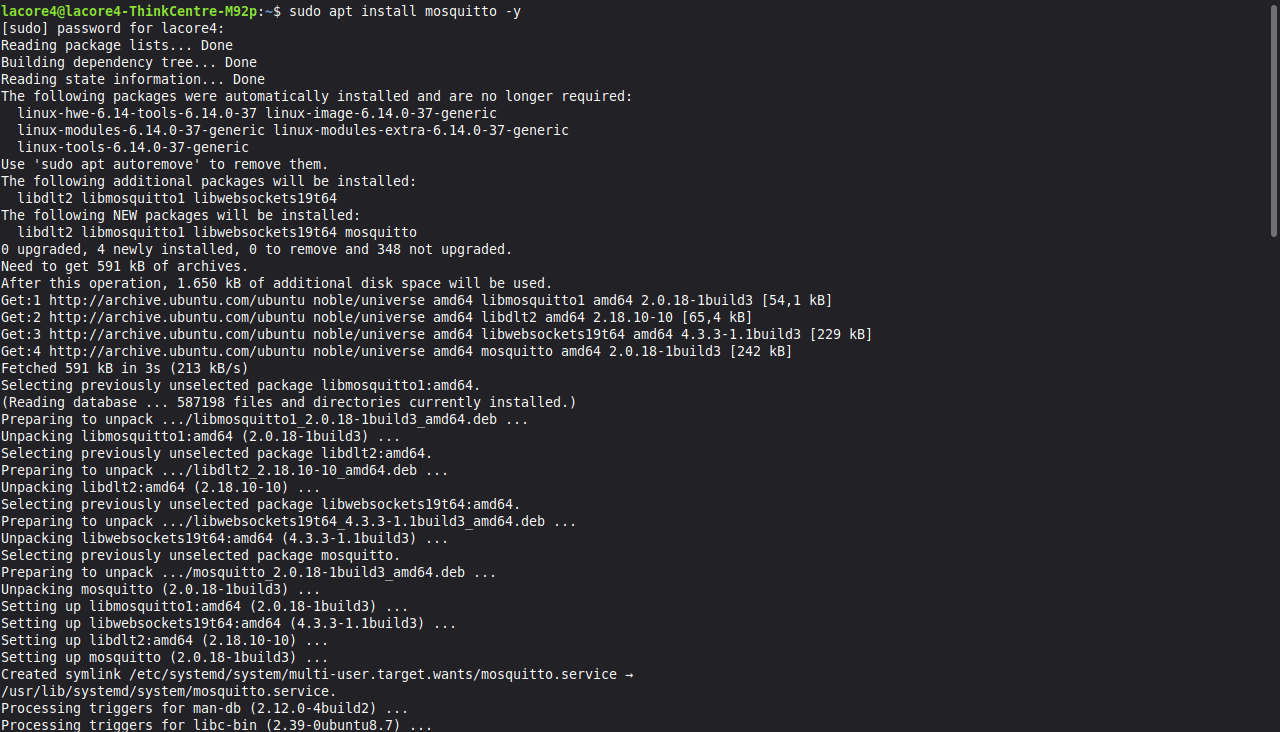
\includegraphics[width=\linewidth]{img/instalacion_broker.png}
    \caption{Instalación del paquete \texttt{mosquitto} y sus dependencias.}
    \label{fig:instalacion_broker}
\end{figure}

\pagebreak

Enseguida se editó el archivo de configuración para declarar puertos y protocolo. La instalación
por defecto de Mosquitto 2.x solo acepta conexiones desde \texttt{localhost}, lo que en este
laboratorio no sirve porque la idea era que otro grupo publicara contra nuestro broker. Por eso
hubo que declarar de forma explícita un \texttt{listener} y permitir clientes anónimos. El
archivo quedó como se muestra en el Código~\ref{lst:conf} y en la
Figura~\ref{fig:config_broker}.

\begin{lstlisting}[language=bash,
    caption={Líneas agregadas a \texttt{/etc/mosquitto/mosquitto.conf}.},
    label={lst:conf},
    float=ht!]
sudo nano /etc/mosquitto/mosquitto.conf

listener 1883                 # puerto por defecto
# habilitar websockets, opcional
listener 9001
protocol websockets
# permitir usuarios anonimos
allow_anonymous true
\end{lstlisting}

\begin{figure}[ht!]
    \centering
    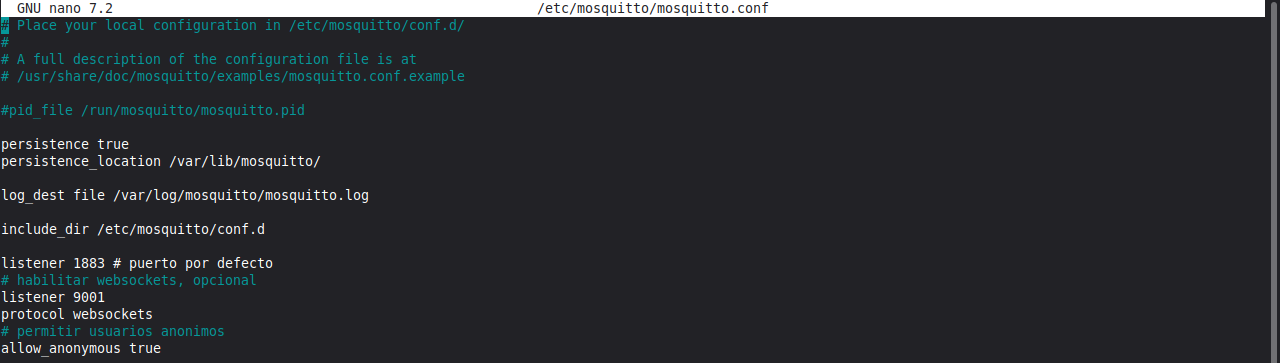
\includegraphics[width=\linewidth]{img/config_broker.png}
    \caption{Archivo de configuración editado con \texttt{nano}.}
    \label{fig:config_broker}
\end{figure}

\pagebreak

Con \texttt{persistence true}, que ya venía en el
archivo, el broker vuelca a disco las suscripciones y los mensajes retenidos, de forma que un
reinicio no borra el estado. \texttt{log\_dest file} manda la bitácora a un archivo en lugar de
dejarla solo en el diario de \texttt{systemd}, lo que facilita revisar conexiones fallidas.
\texttt{include\_dir} hace que todo lo que esté dentro de \texttt{/etc/mosquitto/conf.d} se
cargue después del archivo principal, y esa carpeta es justamente la que se usó más adelante
para la autenticación.

Los dos \texttt{listener} declarados atienden protocolos distintos sobre el mismo broker. El
puerto~1883 es el puerto MQTT estándar sin cifrado~\cite{mqttspec} y es el que usan los clientes
de consola. El puerto~9001 expone el mismo broker sobre WebSockets, que es la vía por la que un
navegador podría suscribirse a un tema sin necesidad de un cliente MQTT nativo.

Antes de reiniciar el servicio se levantó el broker en primer plano contra esa configuración
para comprobar que no tuviera errores de sintaxis, ya que si una directiva está mal escrita
Mosquitto falla al arrancar y el servicio queda caído sin aviso claro.

\begin{lstlisting}[language=bash,
    caption={Verificación de la configuración y arranque del servicio.},
    label={lst:systemctl},
    float=ht!]
sudo mosquitto -c /etc/mosquitto/mosquitto.conf

sudo systemctl start mosquitto
sudo systemctl enable mosquitto
sudo systemctl status mosquitto
\end{lstlisting}

\begin{figure}[ht!]
    \centering
    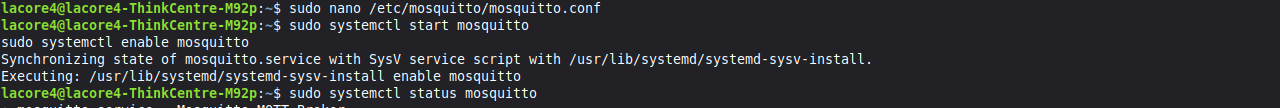
\includegraphics[width=\linewidth]{img/arranque_servicio.png}
    \caption{Arranque del servicio y sincronización con el script SysV.}
    \label{fig:arranque_servicio}
\end{figure}

\pagebreak

El propio paquete crea el enlace simbólico en \texttt{multi-user.target.wants}, de manera que
\texttt{systemd} ya reconoce la unidad apenas termina la instalación. Aun así se ejecutó
\texttt{enable} de forma explícita para dejar constancia de que el broker debe levantarse solo
en cada arranque, y no depender de que alguien lo inicie a mano.

La salida de \texttt{status} confirma el estado \texttt{active (running)} y deja ver algo útil
para entender cómo se comporta el servicio: antes de levantar el proceso principal,
\texttt{systemd} ejecuta cuatro pasos previos de \texttt{ExecStartPre} que crean
\texttt{/var/log/mosquitto} y \texttt{/run/mosquitto} y les asignan el usuario
\texttt{mosquitto}. El proceso corre entonces sin privilegios de administrador, leyendo su
configuración desde \texttt{/etc/mosquitto/mosquitto.conf}
(Figura~\ref{fig:servicio_activo}).

\begin{figure}[ht!]
    \centering
    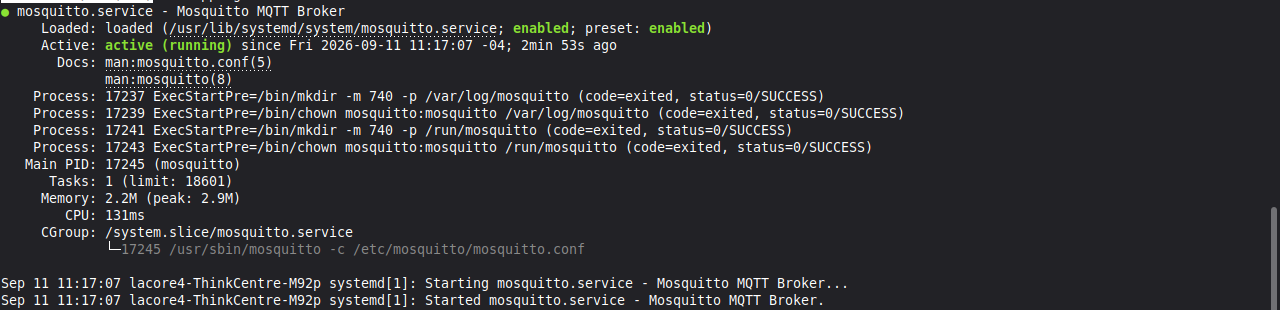
\includegraphics[width=\linewidth]{img/servicio_activo.png}
    \caption{Estado del servicio \texttt{mosquitto.service} tras el arranque.}
    \label{fig:servicio_activo}
\end{figure}

\pagebreak

\textbf{Pasos en la máquina cliente.} El paquete \texttt{mosquitto} solo trae el broker. Las
herramientas de línea de comandos \texttt{mosquitto\_pub} y \texttt{mosquitto\_sub} vienen
aparte, en \texttt{mosquitto-clients}, y se instalaron en los equipos que participaron en la
prueba (Figura~\ref{fig:instalacion_clientes}).

\begin{lstlisting}[language=bash,
    caption={Instalación de los clientes de consola.},
    label={lst:apt_clients},
    float=ht!]
sudo apt install mosquitto-clients -y
\end{lstlisting}

\begin{figure}[ht!]
    \centering
    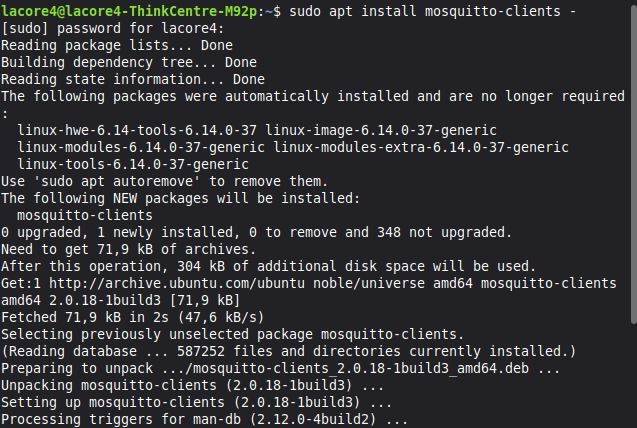
\includegraphics[width=0.9\linewidth]{img/instalacion_clientes.png}
    \caption{Instalación del paquete \texttt{mosquitto-clients}.}
    \label{fig:instalacion_clientes}
\end{figure}

Antes de intentar cualquier publicación se comprobó que hubiera camino de red hasta el equipo
del broker. Esta verificación evita confundir dos problemas muy distintos: que el broker no esté
escuchando, o que el equipo ni siquiera sea alcanzable. Los cinco paquetes ICMP llegaron sin
pérdidas y con tiempos por debajo del milisegundo, lo que descarta el segundo caso
(Figura~\ref{fig:prueba_conectividad}).

\begin{figure}[ht!]
    \centering
    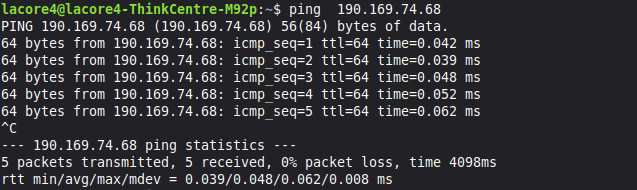
\includegraphics[width=0.9\linewidth]{img/prueba_conectividad.png}
    \caption{Prueba de alcance hacia el equipo que aloja el broker.}
    \label{fig:prueba_conectividad}
\end{figure}

\pagebreak

\textbf{Poniendo a prueba la instalación.} Con el broker escuchando en el puerto~1883 y
aceptando clientes anónimos, la prueba consistió en dejar una terminal suscrita a un tema y
publicar en él desde otra. Se eligió el tema \texttt{kjbhik}, un nombre arbitrario, precisamente
para asegurar que ningún otro grupo estuviera publicando en el mismo espacio de nombres durante
la práctica.

\begin{lstlisting}[language=bash,
    caption={Suscripción y publicación sobre el mismo tema.},
    label={lst:pubsub},
    float=ht!]
# Terminal suscriptora
mosquitto_sub -h 190.169.74.68 -t kjbhik

# Terminal publicadora
mosquitto_pub -h 190.169.74.68 -t kjbhik -m "Prueba exitosa"
\end{lstlisting}

El comportamiento observado deja clara la diferencia con el esquema de sockets del laboratorio
anterior. La terminal suscriptora queda bloqueada esperando, sin conocer quién va a publicar ni
cuántos publicadores hay. La terminal publicadora, por su parte, envía el mensaje y termina de
inmediato, sin saber si alguien estaba escuchando. Cada una de las cinco ejecuciones de
\texttt{mosquitto\_pub} produjo exactamente una línea nueva en el suscriptor
(Figura~\ref{fig:pubsub_anonimo}).

\begin{figure}[ht!]
    \centering
    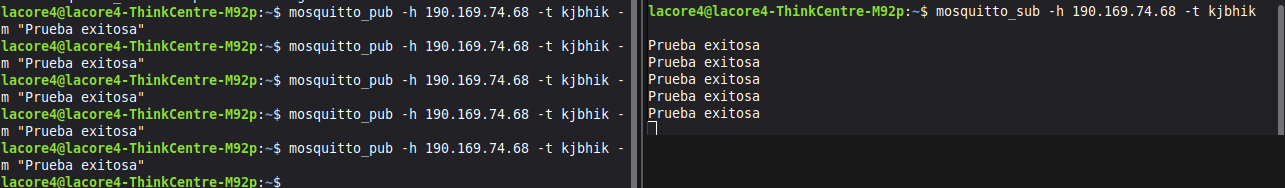
\includegraphics[width=\linewidth]{img/pubsub_anonimo.png}
    \caption{Publicador (izquierda) y suscriptor (derecha) sobre el tema \texttt{kjbhik}.}
    \label{fig:pubsub_anonimo}
\end{figure}

Un detalle que conviene anotar es que los mensajes publicados antes de que el suscriptor se
conectara no aparecen. Sin la bandera \texttt{-r} el broker no retiene el último valor de un
tema, de modo que solo se entrega lo que se publica mientras la suscripción está activa.

\clearpage
%%%%%%%%%%%%%%%%%%%%%%%%%%%%%%%%%%%%%%%%%%%%%%%%%%%%%%%%%%%%%%%%%%%%%%%
\subsection{Autenticación por usuario y clave}

Dejar \texttt{allow\_anonymous true} significa que cualquier equipo de la red puede leer o
escribir en cualquier tema, algo inaceptable en un despliegue real de IoT. El siguiente paso fue
entonces crear un archivo de credenciales con \texttt{mosquitto\_passwd}. La bandera \texttt{-c}
crea el archivo desde cero, por lo que solo debe usarse la primera vez: volver a invocarla borra
los usuarios que ya existían. El alias de usuario elegido fue \texttt{admin}.

\begin{lstlisting}[language=bash,
    caption={Creación del usuario, permisos y reinicio del broker.},
    label={lst:passwd},
    float=ht!]
sudo mosquitto_passwd -c /etc/mosquitto/passwd "admin"
sudo chmod 755 /etc/mosquitto/passwd
sudo systemctl restart mosquitto
\end{lstlisting}

\begin{figure}[ht!]
    \centering
    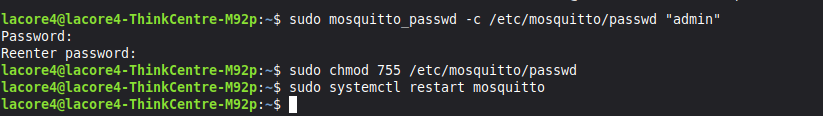
\includegraphics[width=0.9\linewidth]{img/usuario_passwd.png}
    \caption{Creación del usuario \texttt{admin} y reinicio del servicio.}
    \label{fig:usuario_passwd}
\end{figure}

El ajuste de permisos con \texttt{chmod} fue necesario porque el proceso del broker no corre
como administrador, sino con el usuario \texttt{mosquitto}, y sin permiso de lectura sobre el
archivo de contraseñas rechaza todas las conexiones. Hecho esto, se agregaron las dos directivas
de autenticación dentro de \texttt{/etc/mosquitto/conf.d}
(Figura~\ref{fig:config_autenticacion}). Estas líneas se cargan después del archivo principal
gracias al \texttt{include\_dir} configurado antes, de modo que sobrescriben el
\texttt{allow\_anonymous true} original.

\begin{lstlisting}[language=bash,
    caption={Directivas de autenticación.},
    label={lst:conf_auth},
    float=ht!]
allow_anonymous false
password_file /etc/mosquitto/passwd
\end{lstlisting}

\begin{figure}[ht!]
    \centering
    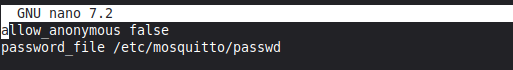
\includegraphics[width=0.55\linewidth]{img/config_autenticacion.png}
    \caption{Directivas de autenticación cargadas desde \texttt{conf.d}.}
    \label{fig:config_autenticacion}
\end{figure}

\pagebreak

\textbf{Poniendo a prueba la instalación.} Tras el reinicio, los mismos comandos de la sección
anterior dejaron de funcionar sin credenciales. Con las banderas \texttt{-u} y \texttt{-P} la
comunicación se restableció y el suscriptor volvió a recibir cada mensaje publicado
(Figura~\ref{fig:pubsub_autenticado}).

\begin{lstlisting}[language=bash,
    caption={Suscripción y publicación autenticadas.},
    label={lst:pubsub_auth},
    float=ht!]
# Terminal suscriptora
sudo mosquitto_sub -h 190.169.74.68 -t test -u "admin" -P "12345"

# Terminal publicadora
sudo mosquitto_pub -h 190.169.74.68 -t test -m "mensaje prueba" -u "admin" -P "12345"
\end{lstlisting}

\begin{figure}[ht!]
    \centering
    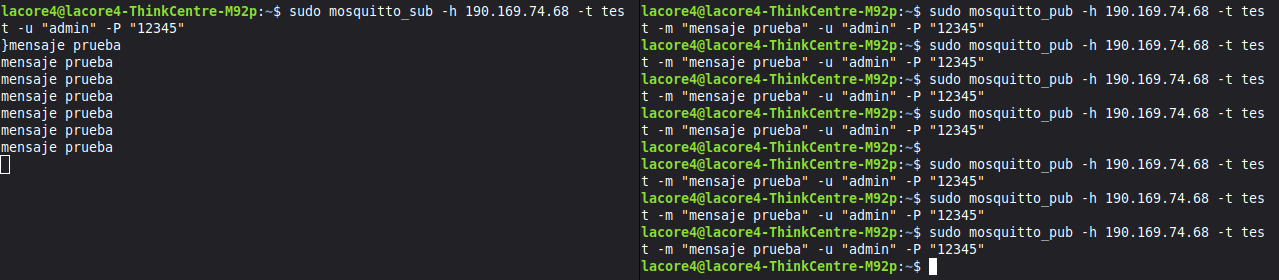
\includegraphics[width=\linewidth]{img/pubsub_autenticado.png}
    \caption{Intercambio autenticado sobre el tema \texttt{test}.}
    \label{fig:pubsub_autenticado}
\end{figure}

Conviene señalar que esta autenticación viaja en claro sobre el puerto~1883. Cualquiera con
acceso al segmento de red puede capturar el usuario y la contraseña con un analizador de
tráfico. En un despliegue real el paso siguiente sería habilitar TLS en el puerto~8883, que es
el puerto reservado para MQTT cifrado.

\clearpage
%%%%%%%%%%%%%%%%%%%%%%%%%%%%%%%%%%%%%%%%%%%%%%%%%%%%%%%%%%%%%%%%%%%%%%%
\section{Conclusiones}

En este laboratorio se pasó de un modelo de comunicación punto a punto a uno mediado por un
broker. La diferencia práctica quedó clara en la prueba de la sección~1.1: el publicador no
necesita saber cuántos suscriptores hay ni si alguno está conectado, y el suscriptor no necesita
saber de dónde viene el dato. Ese desacoplamiento es lo que hace viable una red con muchos
sensores y varios consumidores del mismo dato.

La configuración del broker mostró que Mosquitto 2.x es restrictivo por defecto y solo escucha
en \texttt{localhost}. Declarar el \texttt{listener} de forma explícita no es un detalle
opcional, es lo que permite que el broker sirva a otros equipos de la red.

El mecanismo de \texttt{include\_dir} resultó ser la forma limpia de manejar la configuración.
Mantener la autenticación en un archivo aparte dentro de \texttt{conf.d}, en lugar de editar el
archivo principal, permitió activar y desactivar ese comportamiento sin tocar el resto de las
directivas.

Finalmente, el ajuste de permisos sobre el archivo de contraseñas dejó ver que el broker corre
sin privilegios de administrador. Es un detalle fácil de pasar por alto que se manifiesta como
un rechazo generalizado de conexiones, sin un mensaje que apunte directo a la causa.

\clearpage
%%%%%%%%%%%%%%%%%%%%%%%%%%%%%%%%%%%%%%%%%%%%%%%%%%%%%%%%%%%%%%%%%%%%%%%
\begingroup
\small
\begin{thebibliography}{9}

\bibitem{mqttspec}
A.~Banks, E.~Briggs, K.~Borgendale y R.~Gupta, ``MQTT Version 5.0,''
\emph{OASIS Standard}, mar.~2019. [En línea]. Disponible:
\url{https://docs.oasis-open.org/mqtt/mqtt/v5.0/mqtt-v5.0.html}.
[Consulta: sep.~2026]

\bibitem{mosquittoconf}
Eclipse Foundation, ``mosquitto.conf, the configuration file for mosquitto,''
\emph{Eclipse Mosquitto Documentation}, 2024. [En línea]. Disponible:
\url{https://mosquitto.org/man/mosquitto-conf-5.html}. [Consulta: sep.~2026]

\bibitem{mosquittopasswd}
Eclipse Foundation, ``mosquitto\_passwd, password file generation utility for mosquitto,''
\emph{Eclipse Mosquitto Documentation}, 2024. [En línea]. Disponible:
\url{https://mosquitto.org/man/mosquitto_passwd-1.html}. [Consulta: sep.~2026]

\bibitem{paho}
Eclipse Foundation, ``Eclipse Paho MQTT Python Client,'' 2024. [En línea]. Disponible:
\url{https://eclipse.dev/paho/index.php?page=clients/python/index.php}.
[Consulta: sep.~2026]

\bibitem{guialab}
A.~Russoniello, ``Laboratorio: Protocolo MQTT,'' guía de práctica de laboratorio,
Laboratorio General (Internet de las Cosas), Escuela de Computación,
Facultad de Ciencias, Universidad Central de Venezuela, Caracas, 2026.

\end{thebibliography}
\endgroup

\end{document}
